\documentclass[Rapport/Playerside/RPI_IF/RPI_IF.tex]{subfiles}
\label{sec:playerside_RPI_IF_design}
\begin{document}
\subsubsection{Softwaredesign}
I dette afsnit omtales RPi\_IF boundary klassens design. Klassen er en boundary klasse til RPi og skal stå for at sende cupstatus beskeder til RPi'en, når en ændring forekommer. Den skal også stå for at modtage beskeder fra RPi'en, som kan være en farvekode eller en state ændring. Protokollen brugt er I2C, og til dette formål er en I2C slave komponent brugt i PSoC creators komponent katalog. På figur \ref{fig:I2c_slave} ses denne komponent.
\begin{figure}[H]
    \centering 
    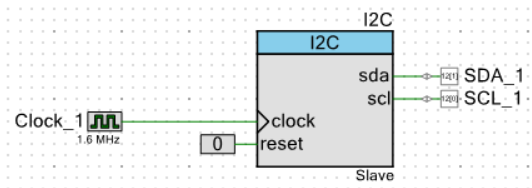
\includegraphics[width=\linewidth]{Softwaredesign/RPI_IF/graphics/i2c_enhed.PNG}
    \caption{I2C slave komponent til kommunikation mellem PSoC playerside og RPi.}
    \label{fig:I2c_slave}
\end{figure}
Denne komponent skal initieres, for at se hvordan dette gøres, ses afsnit \fullref{sec:playerside_RPI_IF_design} i dokumentet design i bilaget. I arkitekturen for denne klasse er to funktioner blevet brugt, som vist i klassediagrammet i figur \ref{fig:CD_PlayerSide} i arkitekturen. Det er sendCupStatus og RPi\_IF\_handledata. Her er sendCupStatus den metode, der står for at sende beskeder omkring cupStatus tilbage til RPi. Funktionen  RPi\_IF\_handledata står for modtagelsen af state ændringer for playerside samt beskeder omkring ændring af farvekode for begge playersides. For en mere detaljeret beskrivelse ses bilaget \textbf{Softwaredesign} i afsnit \fullref{swdesign:sec:RPI_IF_design_bilag}.
\end{document}

